\documentclass[10pt]{book}

\usepackage{times}
\usepackage{graphicx}
\usepackage{url} % for typesetting urls
\usepackage{color}
\usepackage{fancybox}
\usepackage{framed}
\usepackage{hyperref}
\usepackage[super,square]{natbib}
\usepackage{amssymb}
\usepackage{stmaryrd}
\usepackage[a4paper,lmargin=35mm,tmargin=35mm,bmargin=35mm,rmargin=35mm,twoside=false,marginpar=30mm]{geometry}

\newcommand*{\glossfirstformat}[1]{\textit{#1}}
%\usepackage[toc,xindy]{glossaries}
\usepackage[toc]{glossaries}
\makeglossary
%\usepackage[xindy]{imakeidx}
%\makeindex
\renewcommand{\glsdisplayfirst}[4]{\glossfirstformat{#1#4}}

% ===============================================
% A
% ===============================================

% ===============================================
% B
% ===============================================

\newglossaryentry{boolean_expression}{
  name={boolean expression},
  description={An \gls{expression} which evaluates to a value of type \lstinline{bool}}
}

\newglossaryentry{block_comment}{
  name={block comment},
  description={A block comment begins with ``\lstinline{/*}'' and continues until the end-of-comment marker ``\lstinline{*/}''}
}

% ===============================================
% C
% ===============================================

\newglossaryentry{compilation_unit}{
  name={compilation unit},
  description={A single unit of compilation.  In Whiley, this includes
    \gls{source_file}s and also binary \gls{wyil_file}s}
}

% ===============================================
% D
% ===============================================

% ===============================================
% E
% ===============================================

\newglossaryentry{expression}{
  name={expression},
  description={A combination of constants, variables and operators that, when evaluated, produce a single value.  Expressions in certain circumstances may have side effects}
}

% ===============================================
% F
% ===============================================

% ===============================================
% G
% ===============================================

% ===============================================
% H
% ===============================================

% ===============================================
% I
% ===============================================

\newglossaryentry{indentation_syntax}{
  name={indentation syntax},
  description={A lexical organisation of \gls{source_file}s where indentation is significant and is used to group statements and blocks}
}

% ===============================================
% J
% ===============================================

% ===============================================
% K
% ===============================================

% ===============================================
% L
% ===============================================

\newglossaryentry{literal}{
  name={literal},
  description={A source-level entity which describes a value of primitive type}
}

\newglossaryentry{line_comment}{
  name={line comment},
  description={A line comment begins with ``\lstinline{//}'' and continues until the end of line}
}

\newglossaryentry{loop_invariant}{
  name={loop invariant},
  description={A \gls{boolean_expression} which must hold on every iteration of a loop}
}

% ===============================================
% M
% ===============================================

% ===============================================
% N
% ===============================================

% ===============================================
% O
% ===============================================

% ===============================================
% P
% ===============================================

\newglossaryentry{package}{
  name={package},
  description={A unit of hierarchical organisation within the Whiley namespace.}
}

\newglossaryentry{precondition}{
  name={precondition},
  description={A logical condition over the parameters of a function
    or method which must be true immediately prior to execution of
    that function or method.}
}

\newglossaryentry{postcondition}{
  name={postcondition},
  description={A logical condition over the parameters and returns of
    a function or method which must be true immediately after
    execution of that function or method.}  }

% ===============================================
% Q
% ===============================================

% ===============================================
% R
% ===============================================

% ===============================================
% S
% ===============================================

\newglossaryentry{safety_critical_system}{
  name={safety critical system},
  description={A system which operates in a high-risk setting where failure can lead to loss of life, injury, significant damage or environmental harm}
}

\newglossaryentry{source_file}{
  name={source file},
  description={A file in which source code is located.  Source files
    for the Whiley programming language have the extension
    \lstinline{.whiley}.  In Whiley, source files must be compiled into a
    binary form before they can be executed.}
}

\newglossaryentry{statement_block}{
  name={statement block},
  description={A sequence of zero or more consecutive statements with the same indentation}
}

% ===============================================
% T
% ===============================================

\newglossaryentry{type}{
  name={type},
  description={An abstract entity which represents the set of values a given variable may hold, or a given \gls{expression} may evaluate to.}
}

\newglossaryentry{type_descriptor}{
  name={type descriptor},
  description={A source-level description of an underlying \gls{type}.  Unlike many languages, type descriptors and types are quite distinct in Whiley as, for example, two distinct descriptors may describe the same underlying type}
}

\newglossaryentry{type_pattern}{
  name={type pattern},
  description={A source-level description of an underlying \gls{type} (similar to a \gls{type_descriptor}) where one or more variables are associated with its subcomponent(s).}
}


% ===============================================
% U
% ===============================================

% ===============================================
% V
% ===============================================

\newglossaryentry{variable_declaration}{
  name={variable declaration},
  description={A statement which declares one or more variable(s) for use in a given scope.  Each variable is given a \gls{type} which limits the possible values it may hold, and may not already be declared in an enclosing scope}
}

\newglossaryentry{variable_initialiser}{
  name={variable initialiser},
  description={An optional \gls{expression} used to initialise variable(s) declared as part of a \gls{variable_declaration}}
}

\newglossaryentry{verifying_compiler}{
  name={verifying compiler},
  description={A compilers which employs automated mathematical and logical reasoning to check the correctness of the programs that it compiles}
}

% ===============================================
% W
% ===============================================


\newglossaryentry{wyil_file}{
  name={WyIL file},
  description={A compiled (i.e. binary) form of a Whiley \gls{source_file}}
}

% ===============================================
% X
% ===============================================

% ===============================================
% Y
% ===============================================

% ===============================================
% Z
% ===============================================



\usepackage{listings}

% ==========================================
% Whiley LstListing Mode
% ==========================================

\pagestyle{plain}
\lstloadlanguages{Java}
\lstset{
        language=Java,
        keywords={function, method, type, assert, for, while, switch, is, if, case, return,
          else, process, define, as, requires, ensures, where, no,
          all, bool, int, byte, char, string, void, real, in, any, null
        },
        basicstyle=\small\ttfamily,
        commentstyle=\rmfamily\itshape,
        %%Uncomment the following line to avoid boldface keywords
        % keywordstyle=\ttfamily,
        stringstyle=\small\itshape,
        moredelim=*[s][commentstyle]{/*}{*/}, % allows keyword highlighting inside comments
        morecomment=[l][commentstyle]{//},      % single line comments are set by...
        backgroundcolor=\color{lightgray},
        frame=single, % adds a frame around the code
        frameround=tttt,
        framesep=0.25cm,
        texcl,                                                          % ...LaTeX
        moredelim=[is][\ttfamily]{<code>}{</code>}, % allows setting code inside multi-line comments
        moredelim=*[s][\ttfamily]{/*@}{*/}, % JML annotations
        moredelim=*[l][\ttfamily]{//@}, % JML annotations
        moredelim=**[is][\itshape]{/_}{_/}, % allows emphasizing sub-expressions
        moredelim=**[is][\bfseries]{/b_}{_b/}, % allows emphasizing sub-expressions
        escapeinside={(*@}{@*)}, %use (*@\label{line:desc}@*) to label lines for \ref
        mathescape=true,                % allow $ $ for math mode (will this break things?}
        tabsize=4,
	tab=\rightarrowfill,
        xleftmargin=1cm,
        xrightmargin=1cm,
        showspaces=false,
        showtabs=false,
        columns=fullflexible,
        numberstyle=\tiny,
        keepspaces=true,
        mathescape=true, % allows $ to switch in and out of math mode within listings
        literate={->}{{$\rightarrow$}}1 {<<}{{$\langle$}}1 {>>}{{$\rangle$}}1
           {tau}{{$\tau$}}1 {tau'}{{$\tau\prime$}}1 {(|}{{$\lpbar$}}1 {---}{{$\hole$}}1
           {-*-}{{$\times$}}1 {||_}{{$\lceilfloor$}}1 {_||}{{$\rceilfloor$}}1
           {/0}{{$\emptyset$}}1 {/bul}{{$\unit$}}1 {:->}{{$\mapsto$}}1
           {~}{$\sim$}1,
}


\title{\Huge The Whiley Language Specification}

\author{David J. Pearce\\School of Engineering
  and Computer Science\\Victoria University of Wellington, New
  Zealand\\djp@ecs.vuw.ac.nz}

% ======================================================
%\newcommand{\token}[1]{\;\texttt{"#1"}\;}
\definecolor{lightgray}{RGB}{215,215,215}
\definecolor{verylightgray}{RGB}{245,245,245}
\newcommand{\token}[1]{\fcolorbox{black}{lightgray}{\strut\texttt{#1}}}

% --- tokens ---

\newcommand{\nullc}{\token{null}}
\newcommand{\comma}{\token{,}}
\newcommand{\colont}{\token{:}}
\newcommand{\dott}{\token{.}}
\newcommand{\lb}{\token{(}\;}
\newcommand{\rb}{\;\token{)}}
\newcommand{\ra}{\token{=>}}
\newcommand{\lsb}{\token{[}\;}
\newcommand{\rsb}{\;\token{]}}
\newcommand{\lcb}{\token{\{}\;}
\newcommand{\rcb}{\;\token{\}}}
\newcommand{\vbar}{\token{|}}
% ======================================================

% SETUP THE MARGINPAR
\setlength{\marginparwidth}{1cm}
\let\oldmarginpar\marginpar
\renewcommand\marginpar[1]{\-\oldmarginpar[\raggedright\footnotesize #1]%
{\raggedleft\footnotesize #1}}
\newcommand{\hl}[2]{\marginpar{\tiny #1}\colorbox{yellow}{#2}}
%\newcommand{\hl}[2]{#2}

% ======================================================

% \newenvironment{syntax}[1]{
%   \begin{center}
%     \begin{minipage}{0.8\textwidth}
%       \centering
% }{\end{minipage}\end{center}}
\newenvironment{syntax}{
  \def\FrameCommand{\fboxsep=\FrameSep \fcolorbox {black}{verylightgray}}
    \begin{framed}
      \noindent\begin{minipage}{0.9\textwidth}
        \begin{tabular}{rcl}
        }{\end{tabular}\end{minipage}\end{framed}}

% ======================================================

\newtheorem{definition}{Definition}
\newtheorem{lemma}{Lemma}
\newtheorem{corollary}{Corollary}
\newtheorem{theorem}{Theorem}
\newtheorem{proof}{Proof}

% ======================================================

\begin{document}
\maketitle
\tableofcontents

\section{Introduction}
The Whiley programming language has been in active development since
2009.  The language was designed specifically to help the programmer
eliminate bugs from his/her software.  The key feature is that Whiley
allows programmers to write {\em specifications} for their functions,
which are then checked by the compiler.  For example, here is the
specification for the \lstinline{max()} function which returns the
maximum of two integers:

\begin{lstlisting}
function max(int x, int y) => (int z)
// Must return either x or y
ensures x == z || y == z
// Return must be as large as x and y
ensures x <= z ${\tt \&\&}$ y <= z:
    ...
\end{lstlisting}
Here, we see our first piece of Whiley code.  This declares a function
called \lstinline{max} which accepts two integers \lstinline{x} and
\lstinline{y}, and returns an integer \lstinline{z}.  For now, we've
left out the body of this function and put ``\lstinline{...}'' in its
place.  The two \lstinline{requires} clauses form the function's {\em
  post-condition}, which is a guarantee made to any caller of this
function.  In this case, the \lstinline{max} function guarantees to
return one of the two parameters, and that the return will be as large
as both of them.  In plain English, this means it will return the
maximum of the two parameter values.  

When verification is enabled the Whiley compiler will check that every
function meets its specification.  For our \lstinline{max()} function,
this means it will check that body of the function guarantees to
return a value which meets the function's post-condition.  If not, the
compiler will report an error.  The advantage of supporting
specifications, is that they can help uncover bugs and other, more
serious, problems earlier in the development cycle.  This leads to
software which is both more reliable and more easily maintained (since
the specifications provide important documentation).

\subsection{Objectives}

Although the primary purpose of Whiley is to allow us to write
specifications on functions, we will not talk about that again until
the end of the document.  This goal of this article is to introduce
the core language without worrying too much about verification (since
this presents many challenges).  Indeed, it is only once we've
understood the basics of Whiley that we will will be ready to
investigate verification.

\subsection{Installation}

There are currently three ways to get setup with the Whiley
programming language:

\begin{itemize}
\item {\bf Web Browser.} By far the simplest way to get started with
  Whiley is by running it in your web browser (see
  Figure~\ref{whileyplay}).  Go to \url{http://whiley.org/play/} and
  you can get started straight away!
\item {\bf Eclipse Plugin.} If you're familiar with the Eclipse IDE or
  want to develop more serious programs in Whiley, then installing the
  Eclipse plugin is easy to do.  From within Eclipse, choose {\em
    Help$\rightarrow$Install New Software} from the menu.  Enter
  \url{http://whiley.org/eclipse} as the site, select the ``Whiley
  Eclipse Plugin'' and follow the on-screen instructions (see Figure~\ref{wyclipseinstall}).
\item {\bf Development Kit.} For those familiar with the command-line,
  installing the Whiley Development Kit (WDK) is another option.
  Furthermore, you'll be able to explore the source code for the
  Whiley system, and see how it all works!  To do this, visit
  \url{http://whiley.org/downloads/}.
\end{itemize}

More information of getting started with Whiley can be found at
\url{http://whiley.org/getting-started/}.  Finally, the Whiley system
is completely free and released under an open source license (BSD),
and you can get the latest code from \url{http://github.com/Whiley}.

\begin{figure}[!t]
\centering
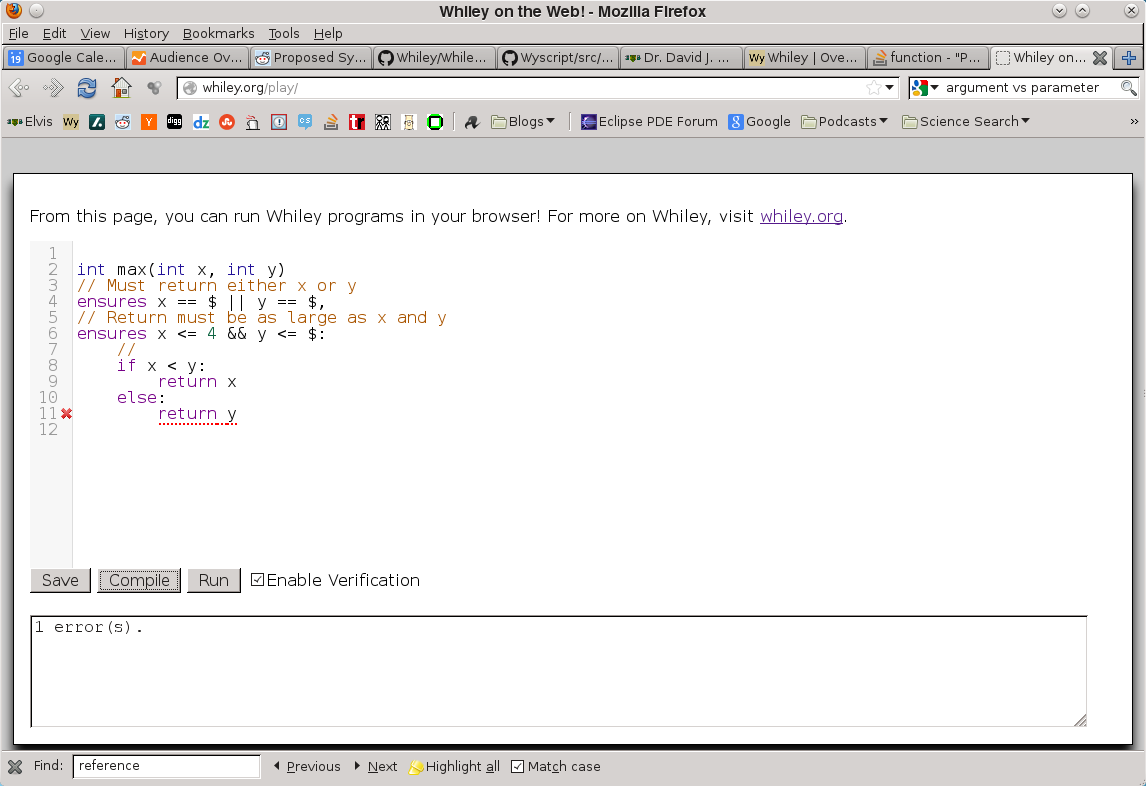
\includegraphics[width=0.9\textwidth]{../images/WhileyPlay.png}
\caption{Compiling a Whiley program using a web browser (Mozilla
  Firefox).  At the moment, the user's program is not correct since
  the system is reporting an error in red.}
\label{whileyplay}
\end{figure}

\begin{figure}[!t]
\centering
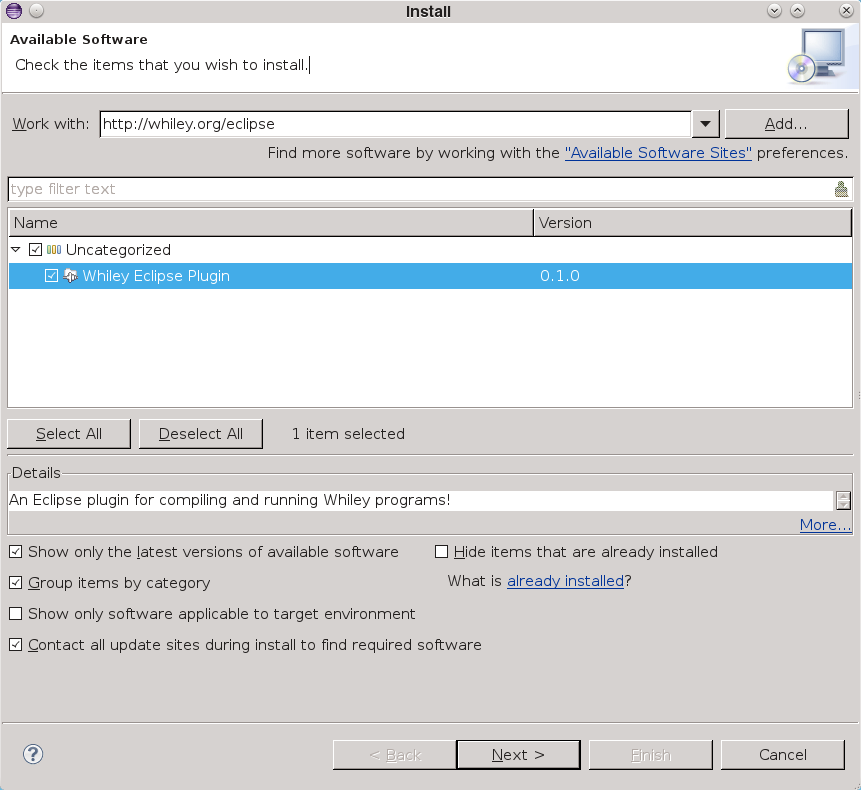
\includegraphics[width=0.9\textwidth]{../images/WyclipseInstallation.png}
\caption{Installing the Whiley Eclipse Plugin from within Eclipse.}
\label{wyclipseinstall}
\end{figure}

\clearpage

\chapter{Lexical Structure}

This chapter specifies the lexical structure of the Whiley programming language.  Programs in Whiley are organised into one or more \gls{source_file}s written in Unicode.  The Whiley language uses \gls{indentation_syntax} to delimit blocks and statements, rather than curly-braces (or similar) as found in many other languages.  

\section{Line Terminators}
A Whiley compiler splits the sequence of (Unicode) input characters into lines by identifying {\em line terminators}:

\begin{syntax}
\verb+LineTerminator+ & $::=$ & \token{\textbackslash n} $|$ \token{\textbackslash r} $|$ \token{\textbackslash r}\ \token{\textbackslash n}\\
\end{syntax}

Here, \token{\textbackslash n} represents the ASCII character \verb+LF+ (\verb+0xA+), whilst \token{\textbackslash r} represents the ASCII character \verb+CR+ (\verb+0xD+).  The two characters \token{\textbackslash r} \token{\textbackslash n} taken together form one line terminator.

\section{Indentation}
After splitting the input characters into lines, a Whiley compiler then identifies the {\em indentation} of each line.  This is necessary because Whiley employs \gls{indentation_syntax} meaning that indentation is significant in the meaning of Whiley programs.  

\begin{syntax}
\verb+Indentation+ & $::=$ & \^\ \big( \token{\textbackslash t} $|$ \token{ }\ \big)$^*$\\
\end{syntax}

Here, \^\ demarcates the start of a line and, hence, indentation may only occur at the beginning of a line.  Indentation may be compared using the $\le$ comparator, such that $i\le ir$ always holds (where $i$ is some indentation and $r$ is either empty or represents additional indentation).  In other words, some indentation $i$ is considered less-than-or-equal to another piece of indentation $ir$ which includes the first as a prefix.  This comparator is important for delimiting \gls{statement_block}s (\S\ref{c_stmts_blocks}).

\pagebreak
\section{Comments}
There are two kinds of comments in Whiley: \gls{line_comment}s and \gls{block_comment}s:
\begin{lstlisting}
/* This is a block comment */
\end{lstlisting}
The above illustrates a block comment, which is all of the text between \token{/*} and \token{*/} inclusive.
\begin{lstlisting}
// This is a line comment
\end{lstlisting}
The above illustrates a line comment, which is all of the text from \token{//} up to the end-of-line.

\section{Identifiers}
An identifier is a sequence of one or more {\em letters} or {\em digits} which starts with a letter.
\begin{syntax}
\verb+Ident+ & $::=$ & \verb+Letter+\ \big(\ \verb+Letter+\ $|$\ \verb+Digit+\ \big)*\\
&&\\
\verb+Letter+ & $::=$ & \token{\_} $|$ \token{a} $|$ \ldots $|$ \token{z} $|$ \token{A} $|$ \ldots $|$ \token{Z}\\
&&\\
\verb+Digit+ & $::=$ & \token{0} $|$ \token{1} $|$ \token{2} $|$ \token{3} $|$ \token{4} $|$ \token{5} $|$ \token{6} $|$ \token{7} $|$ \token{8} $|$ \token{9}\\
\end{syntax}

Letters include lowercase and uppercase alphabetic characters (i.e. \lstinline+a-z+ and \lstinline+A-Z+) and the underscore (\lstinline+_+).

\section{Keywords}
The following strings are reserved for use as {\em keywords} and may not be used as identifiers:

\begin{syntax}
\verb+Keyword+ & $::=$ & \token{all} $|$ \token{any} $|$ \token{assert} $|$ \token{assume} $|$ \token{bool} $|$ \token{break} $|$ \token{byte}\\
         & $|$ & \token{case} $|$ \token{catch} $|$ \token{char} $|$ \token{continue} $|$ \token{debug}\\
         & $|$ & \token{default} $|$ \token{do} $|$ \token{else} $|$ \token{ensures} $|$ \token{export} $|$ \token{false}\\
         & $|$ & \token{finite} $|$ \token{for} $|$ \token{function} $|$ \token{if} $|$ \token{import} $|$ \token{in} $|$ \token{int} $|$ \token{is}\\
         & $|$ & \token{method} $|$ \token{native} $|$ \token{new} $|$ \token{no} $|$ \token{null} $|$ \token{package}\\
         & $|$ &  \token{private} $|$ \token{protected} $|$ \token{public} $|$ \token{real} $|$ \token{requires}\\
         & $|$ & \token{return} $|$ \token{skip} $|$ \token{some} $|$ \token{string} $|$ \token{switch} $|$ \token{throw}\\
         & $|$ & \token{throws} $|$ \token{total} $|$ \token{true} $|$ \token{try} $|$ \token{void} $|$ \token{where} $|$ \token{while}\\
\end{syntax}

The following strings are reserved for use as {\em keywords}, but may additionally be used as identifiers in certain contexts:

\begin{syntax}
\verb+KeywordIdentifier+ & $::=$ & \token{constant} $|$ \token{from} $|$ \token{type}\\
\end{syntax}


\pagebreak

\section{Literals}

A \gls{literal} is a source-level entity which describes a value of primitive type (\S\ref{c_types_primitive_types}).

\begin{syntax}
\verb+Literal+ & $::=$ &  \verb+NullLiteral+ \\
  & $|$ & \verb+BoolLiteral+ \\
  & $|$ & \verb+ByteLiteral+ \\
  & $|$ & \verb+IntLiteral+ \\
  & $|$ & \verb+RealLiteral+ \\
  & $|$ & \verb+CharLiteral+ \\
  & $|$ & \verb+StringLiteral+ \\
\\
\end{syntax}

\subsection{Null Literal}

The \lstinline{null} type (\S\ref{c_types_null}) has a single value expressed as the \lstinline{null} literal.

\begin{syntax}
  \verb+NullLiteral+ & $::=$ & \token{null} \\
\end{syntax}


\subsection{Boolean Literals}

The \lstinline{bool} type (\S\ref{c_types_bool}) has two values expressed as the \lstinline{true} and \lstinline{false} literals.

\begin{syntax}
  \verb+BoolLiteral+ & $::=$ & \token{true} $|$ \token{false} \\
\end{syntax}


\subsection{Byte Literals}

The \lstinline{byte} type (\S\ref{c_types_byte}) has 256 values which are expressed as sequences of binary digits, followed by the suffix ``\lstinline{b}'' (e.g. \lstinline{0101b}).


\begin{syntax}
 \verb+ByteLiteral+ & $::=$ & \big(\ \token{0}\ $|$\ \token{1}\ \big)$^+$\ \token{b}\\
\end{syntax}


Byte literals do not need to contain exactly eight digits and, when fewer digits are given, are padded out to eight digits by appending zero's from the left (e.g. \lstinline{00101b} becomes \lstinline{00000101b}).


\subsection{Integer Literals}

The \lstinline{int} type (\S\ref{c_types_int}) represents the infinite set of integer values which are expressed as sequences of numeric or hexadecimal digits (e.g. \lstinline{123456}, \lstinline{0xffaf}, etc).

\begin{syntax}
  \verb+IntLiteral+ & $::=$ & \big( \token{0}\ $|$\ \ldots\ $|$\ \token{9}\ \big)$^+$ \\
  & $|$ & \token{0} \token{x}\ \big( \token{0}\ $|$\ \ldots\ $|$\ \token{9}\ $|$\ \token{a}\ $|$\ \ldots\ $|$\ \token{f}\ $|$\ \token{A}\ $|$\ \ldots\ $|$\ \token{F}\ \big)$^+$\\
\end{syntax}

Since integer values in Whiley are of arbitrary size (\S\ref{c_types_int}), there is no limit on the size of an integer literal.

\subsection{Real Literals}

The \lstinline{real} type (\S\ref{c_types_real}) represents the infinite set of rational values which are expressed as sequences of numeric digits separated by a period (e.g. \lstinline{1.0}, \lstinline{0.223}, \lstinline{12.55}, etc).

\begin{syntax}
  \verb+RealLiteral+ & $::=$ & \big( \token{0}\ $|$\ \ldots\ $|$\ \token{9}\ \big)$^+$\ \token{.}\ \big( \token{0}\ $|$\ \ldots\ $|$\ \token{9}\ \big)$^+$ \\
\end{syntax}

\subsection{Character Literals}

A {\em character literal} is expressed as a single character or an escape sequence enclosed in single quotes (e.g. \lstinline{'c'}).

\begin{syntax}
  \verb+CharLiteral+ & $::=$ & \token{'}\ \big(\ \verb+Character+\ $|$ \verb+Escape+\ \big)\ \token{'} \\
\end{syntax}

\subsection{String Literals}

A {\em string literal} is expressed as a sequence of zero or more characters or escape sequences enclosed in double quotes (e.g. \lstinline{"Hello World"}).

\begin{syntax}
  \verb+StringLiteral+ & $::=$ & \token{"}\ \big(\ \verb+Character+\ $|$ \verb+Escape+\ \big)$^*$\ \token{"} \\
\end{syntax}

\chapter{Source Files}
\label{c_source_files}
Whiley programs are split across one or more \gls{source_file}s which
are compiled into \gls{wyil_file}s prior to execution.
\Gls{source_file}s contain declarations which describe the functions,
methods, data types and constants which form the program.
\Gls{source_file}s are grouped together into coherent units called
\gls{package}s.


\section{Compilation Units}
\label{c_source_files_compilation_units}
Two kinds of \gls{compilation_unit} are taken into consideration when compiling a Whiley \gls{source_file}: other \gls{source_file}s; and, binary \gls{wyil_file}s.  The Whiley Intermediate Language (WyIL) file format is described elsewhere, but defines a binary representation of a Whiley source file.  When one or more Whiley source files are compiled together, a \gls{compilation_group} is formed.  External symbols encountered during compilation are first resolved from the compilation group, and then from previously \gls{wyil_file}s.

\section{Packages}
\label{c_source_files_packages}

Programs in Whiley are organised into \gls{package}s to help reduce name conflicts and provide some grouping of related concepts.  A Whiley source file may provide an optional \lstinline{package} declaration to identify the package it belongs to.  This declaration must occur at the beginning of the source file.

\begin{syntax}
\verb+PackageDecl+ & $::=$ & \token{package}\ \verb+Ident+\ \big(\ \token{.}\ \verb+Ident+\ \big)$^*$\\
\end{syntax}

Any source file which does not provide a \lstinline{package} declaration is considered to be in the \gls{default_package}.

\section{Names}
\label{c_source_files_names}
There are four functional entities which can be defined within a Whiley source file: \gls{type_declaration}s (\S\ref{c_source_files_type_decl}), \gls{constant_declaration}s (\S\ref{c_source_files_constant_decl}), \gls{function_declaration}s (\S\ref{c_source_files_function_decl}) and \gls{method_declaration}s (\S\ref{c_source_files_method_decl}).  These define {\em named entities} which may be referenced from other \gls{compilation_unit}s.  Every named entity has a unique {\em fully-qualified} name constructed from the enclosing package name, the source file name and the declared name.  For example:\\
\pagebreak

\noindent \verb+Graphics.whiley+
\begin{lstlisting}
package tracer

type Point is { int x, int y }

constant Origin is { x: 0, y: 0 } 
\end{lstlisting}
This declares two named entities: \lstinline{tracer.Graphics.Point} and \lstinline{tracer.Graphics.Origin}.  

Two named entities may {\em clash} if they have the same fully qualified name and are in the same category.  There are three entity categories: {\em types}, {\em constants} and {\em functions/methods}.  The following illustrates a common pattern:

\begin{lstlisting}
type Point is { int x, int y }

function Point(int x, int y) => Point:
    return {x: x, y: y}
\end{lstlisting}

Here, two named entities share the same fully qualified named.  This is permitted because they are in different categories.


\section{Imports}

\section{Declarations}

Camel case

\subsection{Access Control}

% =======================================================================
% Type Declarations
% =======================================================================

\subsection{Type Declarations}
\label{c_source_files_type_decl}

A {\em type declaration} declares a named type within a Whiley
\gls{source_file}.  The declaration may refer to named types in this
or other source filess and may also {\em recursively}
refer to itself (either directly or indirectly).

\begin{syntax}
  \verb+TypeDecl+ & $::=$ & \token{type}\ \verb+Ident+\ \token{is}\
  \verb+TypePattern+\ \big[\ \token{where}\ \verb+Expr+\ \big]\\
\end{syntax}

The optional \lstinline{where} clause defines a
\gls{boolean_expression} which holds for any instance of this type.
This is often referred to as the type {\em invariant} or {\em
  constraint}.  Variables declared within the {\em type pattern} may be
referred to within the optional \lstinline{where} clause.

\paragraph{Examples.}  Some simple examples illustrating type
declarations are:

\begin{lstlisting}
// Define a simple point type
type Point is { int x, int y }

// Define the type of natural numbers
type nat is (int x) where x >= 0
\end{lstlisting}

The first declaration defines an unconstrained record type named
\lstinline{Point}, whilst the second defines a constrained integer
type \lstinline{nat}.

\paragraph{Notes.}  A convention is that type declarations for {\em
  records} or {\em unions of records} begin with an upper case
character (e.g. \lstinline{Point} above).  All other type declarations
begin with lower case.  This reflects the fact that records are most
commonly used to describe objects in the domain.

% =======================================================================
% Constant Declarations
% =======================================================================

\subsection{Constant Declarations}
\label{c_source_files_constant_decl}

A {\em constant declaration} declares a named constant within a Whiley
\gls{source_file}.  The declaration may refer to named constants in this
or other source filess, although it may not refer to itself (either
directly or indirectly).

\begin{syntax}
  \verb+ConstantDecl+ & $::=$ & \token{constant}\ \verb+Ident+\
  \token{is}\ \verb+Expr+\\
\end{syntax}

The given {\em constant expression} is evaluated at {\em compile time}
and must produce a constant value.  This prohibits the use of function
or method calls within the constant expression.  However, general
operators (e.g. for arithmetic) are permitted.

\paragraph{Examples.}  Some example to illustrate constant
declarations are:

\begin{lstlisting}
// Define the well-known mathematical constant to 10 decimal places.
constant PI is 3.141592654

// Define a constant expression which is twice PI
constant TWO_PI is PI * 2.0
\end{lstlisting}

The first declaration defines the constant \lstinline{PI} to have the
\lstinline{real} value \lstinline{3.141592654}.  The second
declaration illustrates a more interesting constant expression which
is evaluated to \lstinline{6.283185308} at compile time.

\paragraph{Notes.}  A convention is that constants are named in upper
case with underscores separating words (i.e. as in \lstinline{TWO_PI}
above).

% =======================================================================
% Function Declarations
% =======================================================================

\subsection{Function Declarations}
\label{c_source_files_function_decl}

A {\em function declaration} defines a function within a Whiley
\gls{source_file}.  Functions are {\em pure} and may not have
side-effects.  This means they are guaranteed to always return the
same result given the same arguments, and are permitted within
specifications (i.e. in type invariants, \gls{loop_invariant}s, and
function/method \gls{precondition}s or \gls{postcondition}s).
Functions may call other functions, but may not call other methods.
They also may not allocate memory on the heap and/or instigate
concurrent computation.

\begin{syntax}
  \verb+FunctionDecl+ & $::=$ & \token{function}\ \verb+Ident+\
  \verb+TypePattern+\ \token{=>}\ \verb+TypePattern+\ \big(\\
  && \ \ \token{throws}\ \verb+Type+\ $|$\ \token{requires}\
  \verb+Expr+\ $|$\ \token{ensures}\ \verb+Expr+\\
  && \big)$^*$\ \token{:}\ \verb+Block+\\
\end{syntax}

The first type pattern (i.e. before "\lstinline{=>}") is referred to
as the {\em parameter}, whilst the second is referred to as the {\em
  return}.  There are three kinds of optional clause which follow:

\begin{itemize}
\item {\bf Throws clause}. This defines the exceptions which may be
  thrown by this function. Multiple clauses may be given, and these
  are taken together as a union. Furthermore, the convention is to
  specify the throws clause before the others.

\item {\bf Requires clause(s)}. These define constraints on the
  permissible values of the parameters on entry to the function or
  method, and are often collectively referred to as the
  \gls{precondition}. These expressions may refer to any variables
  declared within the parameter type pattern. Multiple clauses may be
  given, and these are taken together as a conjunction. Furthermore,
  the convention is to specify the requires clause(s) before any
  ensure(s) clauses.

\item {\bf Ensures clause(s)}. These define constraints on the
  permissible values of the the function or method's return value, and
  are often collectively referred to as the \gls{postcondition}. These
  expressions may refer to any variables declared within either the
  parameter or return type pattern.  Multiple clauses may be given,
  and these are taken together as a conjunction. Furthermore, the
  convention is to specify the requires clause(s) after the others.
\end{itemize}

\paragraph{Examples.}
The following function declaration provides a small example to
illustrate:

\begin{lstlisting}
function max(int x, int y) => (int z)
// return must be greater than either parameter
ensures x <= z && y <= z
// return must equal one of the parmaeters
ensures x == z || y == z:
    // implementation
    if x > y:
        return x
    else:
        return y
\end{lstlisting}

This defines the specification and implementation of the well-known
\lstinline{max()} function which returns the largest of its
parameters. This does not throw any exceptions, and does not enforce
any preconditions on its parameters.

% =======================================================================
% Method Declarations
% =======================================================================

\subsection{Method Declarations}
\label{c_source_files_method_decl}

A {\em method declaration} defines a method within a Whiley
\gls{source_file}.  Methods are {\em impure} and may have
side-effects.  Thus, they cannot be used within specifications
(i.e. in type invariants, \gls{loop_invariant}s, and function/method
\gls{precondition}s or \gls{postcondition}s).  However, unlike
functions, they methods call other functions and/or methods (including
\lstinline{native} methods).  They may also allocate memory on the
heap, and/or instigate concurrent computation.

\begin{syntax}
  \verb+MethodDecl+ & $::=$ & \token{method}\ \verb+Ident+\
  \verb+TypePattern+\ \token{=>}\ \verb+TypePattern+\ \big(\\
  && \ \ \token{throws}\ \verb+Type+\ $|$\ \token{requires}\
  \verb+Expr+\ $|$\ \token{ensures}\ \verb+Expr+\\
  && \big)$^*$\ \token{:}\ \verb+Block+\\
\end{syntax}

The first type pattern (i.e. before "\lstinline{=>}") is referred to
as the {\em parameter}, whilst the second is referred to as the {\em
  return}.  The three optional clauses are defined identically as for
functions above.

\paragraph{Examples.}  The following method declaration provides a
small example to illustrate:

\begin{lstlisting}
// Define the well-known concept of a linked list
type LinkedList is null | { &LinkedList next, int data }

// Define a method which inserts a new item onto the end of the list
method insertAfter(&LinkedList list, int item):
    if *list is null:
        // reached the end of the list, so allocate new node
        *list = new { next: null, data: item }
    else:
        // continue traversing the list
        insertAfter(list->next, item)
\end{lstlisting}





\chapter{Types \& Values}
\section{Overview}
Discuss syntactic versus semantic types, as well as the set of all values.  Probably discuss the different kinds of values which are possible, and the fact that every value has a single {\em concrete} type associate with it.  Also, need to consider constrained types as well as type patterns.

\begin{syntax}
  \verb+Type+ & $::=$ & \\
  & $|$ & \verb+TermType+ \\
  & $|$ & \verb+UnionType+ \\
  & $|$ & \verb+IntersectionType+ \\
\end{syntax}

\begin{syntax}
  \verb+TermType+ & $::=$ & \\
  & $|$ & \verb+PrimitiveType+ \\
  & $|$ & \verb+TupleType+ \\
  & $|$ & \verb+RecordType+ \\
  & $|$ & \verb+ReferenceType+ \\
  & $|$ & \verb+NominalType+ \\
  & $|$ & \verb+CollectionType+ \\
  & $|$ & \verb+NegationType+ \\
  & $|$ & \verb+FunctionType+ \\
  & $|$ & \verb+MethodType+ \\
\end{syntax}


\section{Primitives}

\begin{syntax}
  \verb+PrimitiveType+ & $::=$ & \\
  & $|$ & \verb+AnyType+ \\
  & $|$ & \verb+VoidType+ \\
  & $|$ & \verb+NullType+ \\
  & $|$ & \verb+BoolType+ \\
  & $|$ & \verb+ByteType+ \\
  & $|$ & \verb+CharType+ \\
  & $|$ & \verb+IntType+ \\
  & $|$ & \verb+RealType+ \\
\end{syntax}


% =======================================================================
% Null
% =======================================================================

\subsection{Null Type}

The null type is a special type which should be used to show the absence of something. It is distinct from void, since variables can hold the special \lstinline{null} value (where as there is no special ``\lstinline{void}'' value).  Variables of \lstinline{null} type support only equality (\lstinline{==}) and inequality comparisons (\lstinline{!=}).  The \lstinline{null} value is particularly useful for representing optional values and terminating recursive types.

\begin{syntax}
  \verb+NullType+ & $::=$ & \token{null} \\
\end{syntax}

\paragraph{Examples.}  The following illustrates a simple example of the \lstinline{null} type:

\begin{lstlisting}
type Tree is null | { int data, Tree left, Tree right }

function height(Tree t) => int:
    if t is null:
        // height of empty tree is zero
        return 0
    else:
        // height is this node plus maximum height of subtrees
        return 1 + Math.max(height(t.left), height(t.right))
\end{lstlisting}
This defines \lstinline{Tree} --- a {\em recursive type} --- which is either empty (i.e. \lstinline{null}) or consists of a field \lstinline{data} and two subtrees, \lstinline{left} and \lstinline{right}.  The \lstinline{height} function calculates the height of a \lstinline{Tree} as the longest path from the root through the tree.

\paragraph{Semantics.}  The set of values defined by the type \lstinline{null} is given as follows:
\begin{displaymath}
\begin{array}{rcl}
\llbracket{\tt null}\rrbracket & = & \{{\tt null}\}\\
\end{array}
\end{displaymath}
In other words, the set of values defined by the \lstinline{null} type is the singleton set containing exactly the \lstinline{null} value.


\paragraph{Notes.}  With all of the problems surrounding \lstinline{null} and \lstinline{NullPointerException}s in languages like Java and C, it may seem that this type should be avoided. However, it remains a very useful abstraction around (e.g. for terminating recursive types) and, in Whiley, is treated in a completely safe manner (unlike e.g. Java).

% =======================================================================
% Bool 
% =======================================================================

\subsection{Bool Type}

Represents the set of boolean values (i.e. \lstinline{true} and \lstinline{false}).

\begin{syntax}
 \verb+BoolType+ & $::=$ & \token{bool} \\
\end{syntax}

\paragraph{Examples.}

\paragraph{Semantics.}

\paragraph{Notes.} 

% =======================================================================
% Bool 
% =======================================================================

\subsection{Byte Type}

Represents a sequence of 8 bits. 

\begin{syntax}
 \verb+ByteType+ & $::=$ & \token{byte} \\
\end{syntax}

\paragraph{Examples.}

\paragraph{Semantics.}

\paragraph{Notes.}  Unlike for many languages, there is no
representation associated with a byte. For example, to extract an
integer value from a byte, it must be explicitly decoded according to
some representation (e.g. two's compliment) using an auxillary function (e.g. \lstinline{Byte.toInt()}).


% =======================================================================
% Char
% =======================================================================

\subsection{Char Type}

Represents a arbitrary unicode character.

\begin{syntax}
  \verb+CharType+ & $::=$ & \token{char} \\
\end{syntax}

\paragraph{Examples.}

\paragraph{Semantics.}

\paragraph{Notes.} 

% =======================================================================
% Int
% =======================================================================

\subsection{Int Type}

Represents the set of (unbound) integer values. 

\begin{syntax}
  \verb+IntType+ & $::=$ & \token{int} \\
\end{syntax}

\paragraph{Examples.}

\paragraph{Semantics.}

\paragraph{Notes.}  Since integer types in Whiley are unbounded, there
is no equivalent to Java's \lstinline{MIN_VALUE} and \lstinline{MAX_VALUE} for \lstinline{int} types.

% =======================================================================
% Real
% =======================================================================

\subsection{Real Type}

Represents the set of (unbound) rational numbers.

\begin{syntax}
  \verb+RealType+ & $::=$ & \token{real} \\
\end{syntax}

\paragraph{Examples.}

\paragraph{Semantics.}

\paragraph{Notes.} 

% =======================================================================
% Any
% =======================================================================

\subsection{Any Type}

The type \lstinline{any} represents the type whose variables may hold any possible value.  Thus, \lstinline{any} is the {\em top type} (i.e. $\top$) in the lattice of types and, hence, is the supertype of all other types.  Variables of \lstinline{any} type support only equality (\lstinline{==}) and inequality comparisons (\lstinline{!=}) as well as {\em runtime type tests}.  Finally, unlike the majority of other types, there are no {\em values} of type \lstinline{any}.

\begin{syntax}
  \verb+AnyType+ & $::=$ & \token{any} \\
\end{syntax}

\paragraph{Examples.}  The following illustrates a simple example of the \lstinline{any} type:

\begin{lstlisting}
function toInt(any val) => int:
    if val is int:
        return val
    else if val is real:
        return Math.floor(val)
    else:
        return 0 // default value        
\end{lstlisting}

Here, the function \lstinline{toInt} accepts {\em any valid Whiley value}, which includes all values of type \lstinline{int}, \lstinline{real}, collections, records, etc.  The function then inspects the value that it has been passed and, in the case of values of type \lstinline{int} and \lstinline{real}, returns an integer approximation; for all other values, it returns \lstinline{0}.

\paragraph{Semantics.}  The set of values defined by the type \lstinline{any} is given as follows:
\begin{displaymath}
\begin{array}{rcl}
\llbracket{\tt any}\rrbracket & = & \mathcal{D}\\
\end{array}
\end{displaymath}
In other words, the set of values defined by the \lstinline{any} type equals the {\em domain} (i.e. the set of all values).

\paragraph{Notes.}  The any type is roughly comparable to the \lstinline{Object} type found in pure object-oriented languages.  However, in impure object-oriented languages which support primitive types, such as Java, this comparison often falls short because \lstinline{Object} is not a supertype of primitives such as \lstinline{int} or \lstinline{long}.

% =======================================================================
% Void 
% =======================================================================

\subsection{Void Type}

The \lstinline{void} type represents the type whose variables cannot exist (i.e. because they cannot hold any possible value).  Thus, \lstinline{void} is the {\em bottom type} (i.e. $\bot$) in the lattice of types and, hence, is the {\em subtype} of all other types.  Void is used to represent the return type of a method which does not return anything.  Furthermore, it is also used to represent the element type of an empty list of set.  Finally, unlike the majority of other types, there are no {\em values} of type \lstinline{void}.

\begin{syntax}
   \verb+VoidType+ & $::=$ & \token{void} \\
\end{syntax}

\paragraph{Examples.} The following example illustrates several uses of the \lstinline{void} type:

\begin{lstlisting}
// Attempt to update first element
method update1st(&[int] list, int value) => void:
    // First, check whether list is empty or not
    if *list != [void]:
       // Then, update 1st element
       (*list)[0] = x
    // done
\end{lstlisting}

Here, the method \lstinline{update1st} is declared to return
\lstinline{void} --- meaning it does not return a value.  Instead,
this method updates some existing state accessible through the
reference \lstinline{list}.  Within the method body, the value
accessible via this reference is compared against the
\lstinline{[void]} (i.e. the {\em empty list}).

\paragraph{Semantics.}  The set of values defined by the type
\lstinline{void} is given as follows:
\begin{displaymath}
\begin{array}{rcl}
\llbracket{\tt void}\rrbracket & = & \emptyset\\
\end{array}
\end{displaymath}
In other words, the set of values defined by the \lstinline{void} type
equals the empty set.  

% =======================================================================
% Tuples
% =======================================================================

\section{Tuple Types}

A tuple type describes a compound type made up of two or more subcomponents. It is similar to a record, except that fields are effectively anonymous.

\begin{syntax}
  \verb+TupleType+ & $::=$ & \token{(}\ \verb+Type+\ \big(\ \token{,}\
  \verb+Type+\ \big)$^+$\ \token{)}\\
\end{syntax}

\paragraph{Examples.}

\paragraph{Semantics.}

\paragraph{Notes.}

% =======================================================================
% Records
% =======================================================================

\section{Record Types}

A record is made up of a number of fields, each of which has a unique name. Each field has a corresponding type. One can think of a record as a special kind of "fixed" map (i.e. where we know exactly which entries we have).

\begin{syntax}
  \verb+RecordType+ & $::=$ & \token{\{}\ \verb+Type+\
  \verb+Ident+\ \big(\ \token{,}\ \verb+Type+\ \verb+Ident+\
  \big)$^*$ \big[\ \token{,}\ \token{...}\ \big]\ \token{\}}\\
\end{syntax}

\paragraph{Examples.}

\paragraph{Semantics.}

\paragraph{Notes.}  Syntax for functions?  Open versus closed records?

% =======================================================================
% References
% =======================================================================

\section{Reference Types}

Represents a reference to an object in Whiley.

\begin{syntax}
  \verb+ReferenceType+ & $::=$ & \token{\&}\ \ \verb+Type+\\
\end{syntax}

\paragraph{Examples.}

\paragraph{Semantics.}

\paragraph{Notes.}

% =======================================================================
% Nominal
% =======================================================================

\section{Nominal Types}

The existential type represents the an unknown type, defined at a given position.

\begin{syntax}
  \verb+NominalType+ & $::=$ & \verb+Ident+\\
\end{syntax}

\paragraph{Examples.}

\paragraph{Semantics.}

\paragraph{Notes.}

% =======================================================================
% Collections
% =======================================================================

\section{Collection Types}

% =======================================================================
% Set
% =======================================================================

\subsection{Set Type}

A set type describes set values whose elements are subtypes of the element type. For example, \lstinline|{1,2,3}| is an instance of set type \lstinline|{int}|; however, \lstinline|{1.345}| is not.

\begin{syntax}
  \verb+SetType+ & $::=$ & \token{\{} \ \verb+Type+ \ \token{\}} \\
\end{syntax}

\paragraph{Examples.}

\paragraph{Semantics.}

\paragraph{Notes.} 

% =======================================================================
% Map
% =======================================================================

\subsection{Map Type}

A map represents a one-many mapping from variables of one type to variables of another type. For example, the map type \lstinline|{int=>real}| represents a map from integers to real values. A valid instance of this type might be \lstinline|{1=>1.2,2=>3.0}|.

\begin{syntax}
  \verb+MapType+ & $::=$ & \token{\{} \ \verb+Type+ \ \token{=>} \ \verb+Type+ \ \token{\}} \\
\end{syntax}

\paragraph{Examples.}

\paragraph{Semantics.}

\paragraph{Notes.} 

% =======================================================================
% List
% =======================================================================

\subsection{List Type}

A list type describes list values whose elements are subtypes of the element type. For example, \lstinline{[1,2,3]} is an instance of list type \lstinline{[int]}; however, \lstinline{[1.345]} is not.

\begin{syntax}
  \verb+ListType+ & $::=$ & \token{[} \ \verb+Type+ \ \token{]}\\
\end{syntax}

\paragraph{Examples.}

\paragraph{Semantics.}

\paragraph{Notes.} 

% =======================================================================
% Functions
% =======================================================================

\section{Function Types}

\begin{syntax}
  \verb+FunctionType+ & $::=$ & \token{function}\ \token{(}\
  \big[\ \verb+Type+\ \big(\ \token{,}\ \verb+Type+\ \big)$^*$\ \big]\ \token{)}\ \token{=>}\ \verb+Type+\\
\end{syntax}

\paragraph{Description.}  

\paragraph{Examples.}

\paragraph{Semantics.}

\paragraph{Notes.}

% =======================================================================
% Functions
% =======================================================================

\section{Method Types}

\begin{syntax}
  \verb+MethodType+ & $::=$ & \token{method}\ \token{(}\
  \big[\ \verb+Type+\ \big(\ \token{,}\ \verb+Type+\ \big)$^*$\ \big]\ \token{)}\ \token{=>}\ \verb+Type+\\
\end{syntax}

\paragraph{Description.}  

\paragraph{Examples.}

\paragraph{Semantics.}

\paragraph{Notes.}

% =======================================================================
% Unions
% =======================================================================

\section{Union Types}

A union type represents a type whose variables may hold values from any of its "bounds". For example, the union type \lstinline{null|int} indicates a variable can either hold an integer value, or \lstinline{null}. 

\begin{syntax}
  \verb+UnionType+ & $::=$ & \verb+IntersectionType+\ \big(\ \token{|}\ \verb+IntersectionType+\
  \big)$^+$\\
\end{syntax}

\paragraph{Examples.}

\paragraph{Semantics.}

\paragraph{Notes.}  There must be at least two bounds for a union type to make sense.

% =======================================================================
% Intersections
% =======================================================================

\section{Intersection Types}

\begin{syntax}
  \verb+IntersectionType+ & $::=$ & \verb+TermType+\ \big(\ \token{\&}\ \verb+TermType+\
  \big)$^+$\\
\end{syntax}

\paragraph{Description.}

\paragraph{Examples.}

\paragraph{Semantics.}

\paragraph{Notes.}

% =======================================================================
% Negations
% =======================================================================

\section{Negation Types}

\begin{syntax}
  NegationType & $::=$ & \token{!}\ \ \verb+Type+\\
\end{syntax}

\paragraph{Description.}  A negation type represents a type which
accepts values {\em not} in a given type.

\paragraph{Examples.}

\paragraph{Semantics.}

\paragraph{Notes.}

\section{Abstract Types}
\subsection{Recursive Types}
\subsection{Effective Tuples}
\subsection{Effective Records}
\subsection{Effective Collections}

\section{Subtyping Algorithms}
Discussion of soundness and completeness.

\chapter{Statements}

% =======================================================================
% AssertStatement
% =======================================================================

\section{Assert Statement}

Represents an {\em assert statement} of the form ``\lstinline{assert e}'', where \lstinline{e} is a \gls{boolean_expression}. 

\begin{syntax}
  \verb+AssertStmt+ & $::=$ & \token{assert}\ \verb+Expr+\\
\end{syntax}

\paragraph{Examples.} The following illustrates:
\begin{lstlisting}
function abs(int x) => int:
    if x < 0:
        x = -x
    assert x >= 0
    return x
\end{lstlisting}

\paragraph{Notes.}  Assertions are either {\em statically checked} by the
verifier, or turned into {\em runtime checks}.


% =======================================================================
% Assignment Statement
% =======================================================================

\section{Assignment Statement}

Represents an {\em assignment statement} of the form \lstinline{lhs = rhs}.  Here, the \lstinline{rhs} is any expression, whilst the \lstinline{lhs} must be an \lstinline{LVal} --- that is, an expression permitted on the left-side of an assignment.

\begin{syntax}
  \verb+AssignStmt+ & $::=$ & \verb+LVal+\ \token{=}\ \verb+Expr+\\
\end{syntax}


\paragraph{Examples.} The following illustrates different possible assignment statements:
\begin{lstlisting}
x = y       // variable assignment
x.f = y     // field assignment
x[i] = y    // list assignment
x[i].f = y  // compound assignment
\end{lstlisting}

The last assignment here illustrates that the left-hand side of an
assignment can be arbitrarily complex, involving nested assignments
into lists and records.

\paragraph{Semantics.}

\paragraph{Notes.} 

% =======================================================================
% Assume Statement
% =======================================================================

\section{Assume Statement}

Represents an {\em assume statement} of the form ``\lstinline{assume e}'', where \lstinline{e} is a \gls{boolean_expression}.

\begin{syntax}
  \verb+AssumeStmt+ & $::=$ & \token{assume}\ \verb+Expr+\\
\end{syntax}


\paragraph{Examples.}  The following illustrates a simple function
which uses an \lstinline{assume} statement to meet its
postcondition:

\begin{lstlisting}
function abs(int x) => int:
    assume x >= 0
    return x
\end{lstlisting}

\paragraph{Notes.} Assumptions are {\em assumed} by the verifier and, since
this may be unsound, are always turned into {\em runtime checks}.

% =======================================================================
% ReturnStatement
% =======================================================================

\section{Return Statement}

Represents a {\em return statement} with an optional expression is referred to as the {\em return value}.

\begin{syntax}
  \verb+ReturnStmt+ & $::=$ & \token{return}\ \big[\ \verb+Expr+\
  \big]\\
\end{syntax}

\paragraph{Examples.} The following illustrates a simple function
which returns the increment of its parameter \lstinline{x}:

\begin{lstlisting}
function f(int x) => int:
    return x + 1
\end{lstlisting}

Here, we see a simple \lstinline{return} statement which returns an \lstinline{int} value.

\paragraph{Notes.}  The returned expression (if there is one) must
begin on the same line as the return statement itself.

% =======================================================================
% ThrowStatement
% =======================================================================

\section{Throw Statement}

\begin{syntax}
  \verb+ThrowStmt+ & $::=$ & \token{throw}\ \verb+Expr+\\
\end{syntax}

\paragraph{Description.}

\paragraph{Examples.}

\paragraph{Notes.} 

% =======================================================================
% Variable Declarations
% =======================================================================

\section{Variable Declarations}

Represents a \gls{variable_declaration} which has an optional expression assignment referred to as an \gls{variable_initialiser}.  If an initialiser is given, then this will be evaluated and assigned to the variable when the declaration is executed.

\begin{syntax}
  \verb+VarDecl+ & $::=$ & \verb+Type+\ \verb+Ident+\ \big[\
  \token{=}\ \verb+Expr+\ \big]\\
\end{syntax}

\paragraph{Examples.} Some example variable declarations are:
\begin{lstlisting}
int x
int y = 1
int z = x + y
\end{lstlisting}

\paragraph{Notes.} 


% =======================================================================
% If Statement
% =======================================================================

\section{If Statement}

Represents a classical \lstinline{if} statement which supports
chaining and an optional \lstinline{else} branch.  The expression(s)
are referred to as {\em conditions} and must be
\gls{boolean_expression}s.  The first block is referred to as the {\em
  true branch}, whilst the optional \lstinline{else} block is referred to as the {\em false branch}.

\begin{syntax}
  \verb+IfStmt+$^\ell$ & $::=$ & \token{if}\ \verb+Expr+\ \token{:}
  \verb+Block+$^\gamma$\ \big( \token{else} \token{if}\ \verb+Expr+\ \token{:}
  \verb+Block+$^{\omega_i}$\ \big)$^*$ \\
&& \big[ \token{else} \token{:} \verb+Block+$^\phi$\ \big]\\
&&\\
\multicolumn{3}{r}{(where $\ell < \gamma$ and $\forall i.\ell <
  \omega_i$ and $\ell < \phi$)}\\
\end{syntax}

\paragraph{Examples.} The following illustrates:

\begin{lstlisting}
function max(int x, int y) => int:
    if(x > y):
        return x
    else if(x == y):
        return 0
    else:
        return y
\end{lstlisting}

\paragraph{Notes.} 

% =======================================================================
% While Statement
% =======================================================================

\section{While Statement}

Represents a while statement with optional \lstinline{where} clause(s) commonly referred to as \gls{loop_invariant}s.

\begin{syntax}
  \verb+WhileStmt+$^\ell$ & $::=$ & \token{while}\ \verb+Expr+\ \big(\
  \token{where}\ \verb+Expr+\ \big)$^*$\ \token{:}\ \verb+Block+$^\gamma$\ \\
&&\\
\multicolumn{3}{r}{(where $\ell < \gamma$)}\\
\end{syntax}

\paragraph{Examples.} As an example:

\begin{lstlisting}
function sum([int] xs) => int:
  int r = 0
  int i = 0
  while i < |xs| where i >= 0:
    r = r + xs[i]
    i = i + 1
  return r
\end{lstlisting}

\paragraph{Notes.}   When multiple \lstinline{where} clauses are
given, these are combined using a conjunction. The combined invariant
defines a condition which must be true on every iteration of the loop.

% =======================================================================
% Do/While Statement
% =======================================================================

\section{Do/While Statement}

\begin{syntax}
  \verb+DoWhileStmt+$^\ell$ & $::=$ & \token{do}\ \token{:}
  \verb+Block+$^\gamma$\ \token{while}\ \verb+Expr+\ \big(\
  \token{where}\ \verb+Expr+\ \big)$^*$\\
&&\\
\multicolumn{3}{r}{(where $\ell < \gamma$)}\\
\end{syntax}

\paragraph{Description.}

\paragraph{Examples.}

\paragraph{Notes.} 

% =======================================================================
% For Statement
% =======================================================================

\section{For Statement}

\begin{syntax}
  \verb+ForStmt+$^\ell$ & $::=$ & \token{for}\ \verb+VarPattern+\
  \token{in}\ \verb+Expr+\ \big(\ \token{where}\ \verb+Expr+\
  \big)$^*$\ \token{:} \verb+Block+$^\gamma$\\
&&\\
\multicolumn{3}{r}{(where $\ell < \gamma$)}\\
\end{syntax}

\paragraph{Description.}

\paragraph{Examples.}

\paragraph{Notes.} 

% =======================================================================
% Switch Statement
% =======================================================================

\section{Switch Statement}

\begin{syntax}
  \verb+SwitchStmt+ & $::=$ &\\
\end{syntax}

\paragraph{Description.}

\paragraph{Examples.}

\paragraph{Notes.} 

% =======================================================================
% Try/Catch Block
% =======================================================================

\section{Try/Catch Statement}

\begin{syntax}
  \verb+TryCatchStmt+ & $::=$ &\\
\end{syntax}

\paragraph{Description.}

\paragraph{Examples.}

\paragraph{Notes.} 

\chapter{Expressions}
\Gls{expression} blah blah.

\section{Binary Expressions}
\begin{figure}[!t]
  \centering
  \fbox{
    \begin{tabular}{rcll}
      Expr & $::=$ & $ Cond\;[\;(\;\token{\&\&}\;|\;\token{||}\;)\;Expr\;] $ & {\em // Expressions}\\
      &&&\\
      Cond & $::=$ & $ Append\;[\;Cop\;Expr\;] $ & {\em // Condition Expressions}\\
      &&&\\
      Append & $::=$ & $ Range\;[\;\token{++}\;Expr\;] $ & {\em // Append Expressions}\\
      &&&\\
Range & $::=$ & $ AddSub\;[\;\token{..}\;Expr\;] $ & {\em // Range Expressions}\\
&&&\\
AddSub & $::=$ & $
MulDiv\;[\;(\;\token{+}\;|\;\token{-}\;)\;Expr\;] $ & {\em //
  Additive Expressions}\\
&&&\\
MulDiv& $::=$ & $
Index\;[\;(\;\token{*}\;|\;\token{/}\;|\;\token{\%}\;)\;Expr\;] $ & {\em //
Multiplicative Expressions}\\

&&&\\
Index& $::=$ & ??? & {\em //
Index Expressions}\\
\end{tabular}}
\caption{Syntax for Binary Expressions}
\end{figure}



\begin{figure}[!t]
\centering
\fbox{
\begin{tabular}{rcll}
Term& $::=$ & {\em // Terms} \\
&{\huge\strut}$|$& $Constant$ & {\em // Constant expressions}\\
&{\huge\strut}$|$& $Identifier$ & {\em // Identifier expressions}\\
&{\huge\strut}$|$&$ Expr_1\;(\;\comma\;Expr_i\;)^+$ & {\em // Tuple expressions}\\

&{\huge\strut}$|$&$ \lb Expr \rb $ & {\em // Bracketed expressions}\\

&{\huge\strut}$|$&$ \vbar\;Expr\;\vbar  $ & {\em // Size expressions}\\

&{\huge\strut}$|$&$ Identifier\;\lb\;[\;Expr_1\;(\;\comma\;Expr_i\;)^+\;]\;\rb $ & {\em // Invocation expressions}\\

&{\huge\strut}$|$&$
(\;\token{-}\;|\;\token{!}\;|\;\token{\~}\;|\;\token{\&}\;|\;\token{*}\;)\;Expr
$ & {\em // Unary expressions}\\

&{\huge\strut}$|$&$ \token{new}\;Expr $ & {\em // Allocation expressions}\\

&{\huge\strut}$|$&$ \lcb [\;Expr_1\;(\;\comma\;\;Expr_i\;)^*\;]\rcb $ & {\em
  // Set expressions}\\

&{\huge\strut}$|$&$ \lcb [\;Expr_1\:\token{=>}\:Expr'_1\;(\;\comma\;\;Expr_i\:\token{=>}\:Expr'_i\;)^*\;]\rcb $ & {\em
  // Map expressions}\\

&{\huge\strut}$|$&$ \lsb [\;Expr_1\;(\;\comma\;\;Expr_i\;)^*\;]\rsb $ & {\em // List expressions}\\

&{\huge\strut}$|$&$ \lcb [\;n_1\colont\;Expr_1\;(\;\comma\;\;n_i\;\colont\;Expr_i\;)^*\;]\rcb $ & {\em // Record expressions}\\
\end{tabular}}
\caption{Syntax for Term Expressions}
\end{figure}


\begin{figure}[!t]
\centering
\fbox{
\begin{tabular}{rcll}
Constant& $::=$ & {\em // Constants} \\
&{\Huge\strut}$|$&$ (\;\token{0}\;|\;\token{1}\;)^+\;\token{b} $ & {\em // Boolean constants}\\

&{\Huge\strut}$|$&$ (\;\token{0-9}\;)^+ $ &
{\em // Integer constants}\\

&{\Huge\strut}$|$&$ (\;\token{0-9}\;)^+\;\dott\;(\;\token{0-9}\;)^+$ &
{\em // Decimal constants}\\

&{\Huge\strut}$|$& $\nullc$ & {\em // Null constant}\\
\end{tabular}}
\caption{Syntax for Constant Expressions}
\end{figure}

\begin{figure}[!t]
\centering
\fbox{
\begin{tabular}{rcll}
Identifier& $::=$ & $ (\;\token{\_}\;|\;\token{a-z}\;|\;\token{A-Z}\;)\;(\;\token{\_}\;|\;\token{a-z}\;|\;\token{A-Z}\;|\;\token{0-9}\;)^* $ & {\em // Identifiers}\\


\end{tabular}}
\caption{Syntax for Identifiers}
\end{figure}


\newpage
\section{Flexible Types}
The previous section introduced us to the basic types found in Whiley,
such as integers (\lstinline{int}), rationals (\lstinline{real}) and
booleans (\lstinline{bool}).  However, unlike many languages, Whiley
provides a flexible and powerful approach to typing which go well
beyond the basic forms.  In this section, we will examine this in more
detail.

\subsection{Flow Typing}
To improve the programmer experience and reduce unnecessary tedium,
Whiley employs a {\em flow typing} system.  What this means is that
the type of a variable can vary at different points within a function.
To make this work, Whiley employs {\em union types}~\cite{BC91,IN07} along with {\em variable retyping}.  The
following example illustrates how this works (where the body of
\lstinline{indexOf()} is left out for brevity):

\begin{lstlisting}
 function indexOf(string str, char c) => null|int:
    ...

 function split(string str, char c) => [string]:
    var idx = indexOf(str,c)
    // idx has type null$|$int
    if idx is int:
        // idx now has type int
        int below = str[0..idx]
        int above = str[idx..]
        return [below,above]
    else:
        // idx now has type null
        return [str] // no occurrence
\end{lstlisting}
Here, \lstinline{indexOf()} returns the first index of a character in
the string, or \lstinline{null} if there is none.  The type
\lstinline{null|int} is a {\em union type}, meaning it is either an
\lstinline{int} or \lstinline{null}.  The \lstinline{split()} function
splits a string into two pieces based on the first occurrence of a
given character \lstinline{c}, or leaves the string as is otherwise.
It calls \lstinline{indexOf()} to determine the first occurrence of
\lstinline{c} in \lstinline{str}.  Observe that variable
\lstinline{idx} has been declared as type \lstinline{var}, meaning the
compiler will automatically infer the best possible type for it.

In the above example, Whiley's flow typing system seamlessly ensures
that \lstinline{null} is never dereferenced.  This is because the type
\lstinline{null|int} cannot be treated as an \lstinline{int}.
Instead, one must first check it is an \lstinline{int} using a type
test, such as ``\lstinline{idx is int}''.  Whiley automatically
{\em retypes} \lstinline{idx} to \lstinline{int} when this is known to be
true, thereby avoiding any awkward and unnecessary syntax (e.g. a cast
as required in many languages).

\begin{insight}{Null References.}  In many languages (e.g. C/C++,
  Java, etc) the use of \lstinline{null} is a significant source of
  error (see e.g.~\cite{Hoa09}).  For example, in Java dereferencing
  the \lstinline{null} value gives rise to a
  \lstinline{NullPointerException}, which is regarded as the most
  common form of error in Java~\cite{XYZ}.  The issue is that, in such
  languages, one can treat {\em nullable} references as though they
  are {\em non-null} references~\cite{Pier02}.  In the research
  literature, there have been many proposals to solve this problem
  using static type systems
  (e.g.~\cite{PQVHV01,FL03,KH07,CFJJ06,CJ07,MPPD08,Hub08,HJP08}).
  Unfortunately, at the time of writing, very few languages have
  incorporated such ideas.
\end{insight}

\begin{insight}{Intersections and Negations.}
  Whiley also supports so-called {\em intersection} and {\em negation}
  types.  Whilst these can be expressed directly in source code, they
  are generally less useful than unions.
\end{insight}

\begin{insight}{Untagged Unions}.  Often confusion surrounding untagged
    versus tagged unions.  The latter are more common, and sometimes
    known as {\em sum types}.
\end{insight}

\subsection{Recursive Types}
To represent tree-like structures, Whiley provides {\em recursive
  types} which are similar to the algebraic data types found in
functional languages (e.g. Haskell, ML, etc).  For example:
\begin{lstlisting}
// A linked list is either the empty list or a link
type LinkedList is EmptyList | Link

// The empty list contains no links
type EmptyList is null

// A single link in a linked list
type Link is {int data, LinkedList next}

// Return the length of a linked list (i.e. the number of links it contains)
int length(LinkedList l):
  if l is null:    
    return 0 // l now has type null
  else:    
    return 1 + length(l.next) // l now has type \{int data, LinkedList next\}
\end{lstlisting}
Here, \lstinline{LinkedList} is a recursive type representing a linked
list (i.e. a sequence of zero or more links).  The empty list is
defined as \lstinline{null}, whilst each link contains a
\lstinline{data} field.  The type \lstinline{LinkedList} is defined in
terms of itself (i.e. it is recursive) and describes linked lists of
arbitrary size.

\begin{insight}{Value Semantics.}
  As discussed in \S\ref{value_semantics} all compounds structures in
  Whiley are passed by value, {\em including recursive types}.  This
  differs from common languages (e.g. Java), where linked structures
  are typically composed from {\em references} to link objects.  This
  means, for example, that linked structures in such languages can
  share substructures, leading to subtle and hard-to-find bugs.  In
  Whiley linked structures, such as \lstinline{LinkedList}, can never
  share substructure.
\end{insight}

The above example also serves as another illustration of flow typing
in Whiley.  More specifically, on the false branch of the type test
``\lstinline{l is null}'', variable \lstinline{l} is automatically
retyped to \lstinline+{int data, LinkedList next}+ --- thus ensuring
the subsequent dereference of \lstinline{l.next} is safe.  No casts
are required as would be needed for a conventional imperative language
(e.g. Java).  Finally, like all compound structures, the semantics of
Whiley dictates that recursive data types are passed by value (or, at
least, appear to be from the programmer's perspective).

%\subsection{Polymorphism \& Encapsulation}
%Two important hallmarks of the object-oriented paradigm are
%polymorphism and encapsulation.  The former is typically achieved
%through inheritance and/or interfaces, whilst the latter typically
%exploits \lstinline{public} / \lstinline{private} modifiers.  Whiley
%does not permit \lstinline{public} or \lstinline{private} modifiers in
%records.  Instead, Whiley employs a simple form of {\em existential
%type}~\cite{}, illustrated as follows:
%
%\begin{lstlisting}
% define Shape as { 
%   bool contains(int x, int y, Shape this), 
%   ... 
% }
%\end{lstlisting}
%This declares what is, essentially, an interface.  The
%``\lstinline{...}''  notation is significant here, as it denotes
%unknown --- or {\em existential} --- state~\cite{Cook09}.  We can then
%``implement'' this interface as follows:
%
%\begin{lstlisting}
% define Square as {
%   int x, int y, int width, int height,   
%   bool contains(int x, int y, Square this)
% }
%
% bool defSqContains(int x, int y, Square sq):
%     if x >= sq.x && x < (sq.x + sq.width):
%         return y >= sq.y && 
%                y < (sq.y + sq.height)
%     return false
%
% Square defSquare(int x, int y, int w, int h):
%     return {x: x, y: y, width: w, height: h,
%             contains: &defSqContains}
%\end{lstlisting}
%{\bf THIS NEEDS WORK --- IT'S BROKEN}

\subsection{Structural vs Nominal Types}
Statically typed languages, such as Java, employ {\em nominal typing}
for recursive data types.  This means that two otherwise identical
types with different names are considered distinct and, for example, a
variable of one type cannot flow into the other.  In contrast, Whiley employs {\em structural typing} of records~\cite{Card88} to give greater flexibility.  This means that the name of a type is, generally speaking, unimportant.  Instead, identical types (i.e. those with identical {\em structure}) with different names are still considered identical in Whiley.  For example:

\begin{lstlisting}
// Define the notion of a "rectangle"
type Rectangle is { int x, int y, int width, int height }
// Define the notion of a "bounding box"
type BoundingBox is { int x, int y, int width, int height }

// Define a function for computing the area of a rectangle
function area(Rectangle rect) => int:
    return rect.width * rect.height
\end{lstlisting}

In this example, the types \lstinline{Rectangle} and \lstinline{BoundingBox} are {\em identical} and can be used interchangeably.  For example, if we have a variable of type \lstinline{BoundingBox}, we can safely pass it to the \lstinline{area()} function above to compute its area.

\subsubsection{Nominal Types}

It is possible to simulate nominal types in Whiley.

\subsection{Subtyping}

An important concept in many modern programming languages is that of {\em subtyping}.  This defines a relationship between otherwise different types (i.e. which do not have identical structure).  

\subsection{Coercions}

A {\em coercion} converts a value of one type into a corresponding value of another type.  For example, in Whiley, we can coerce the \lstinline{int} value ``\lstinline{0}'' into the \lstinline{real} value ``\lstinline{0.0}''.  Many programming languages permit both {\em implicit} and {\em explicit} coercions, with the latter more commonly referred to as {\em casting}.  Implicit coercions occur without explicit direction from the programmer, and are often considered dangerous because of this.  

\begin{insight}{Lossless Coercions?}
The Java programming language attempts to enforce a requirement that implicit coercions are {\em lossless}.  Thus, any coercion which may result in a loss of information must be made explicit through the use of a cast.  Unfortunately, Java does permit implicit lossy coercions by, for example, allowing \lstinline{int} values to be implicitly coerced into \lstinline{float} values --- because not every \lstinline{int} value can be represented by a \lstinline{float} in Java.
\end{insight}

To address the issues surrounding implicit coercions, Whiley only permits implicit coercions which are lossless.  That is, which do not result in a loss of information.  In contrast, {\em lossy} coercions require an explicit cast be used to ``force'' the coercion.  The following example illustrates:
\begin{lstlisting}
type Link is {int data, LinkedList next}
type LinkedList is null | Link
type OrderedList is null | {
  int data, int order, OrderedList next
}
\end{lstlisting}
Here, we have defined a standard linked list and a specialised
``ordered'' list.  The intuition is that \lstinline{order < next.order} for each node in an \lstinline{OrderedList} (although the details of how this is done are unimportant here).   These two types are not considered identical because they have different structure (i.e. \lstinline{OrderedList} has an additional field, \lstinline{order}).  However, there is still a subtyping relationship between them (i.e. \lstinline{OrderedList} subtypes \lstinline{LinkedList}).  Thus, an instance of \lstinline{OrderedList} can be used where a \lstinline{LinkedList} was expected.  For example:

\begin{lstlisting}
function sum(LinkedList l) => int:
    if l is null:
        return 0
    else:
        return l.data + sum(l.next)
\end{lstlisting}

This defines a simple recursive function for computing the length of a \lstinline{LinkedList}.  Instances of \lstinline{OrderedList} can be passed into this function by {\em coercing} them to instances of \lstinline{LinkedList}:

\begin{lstlisting}
function sum(OrderedList l) => int:
    return sum((LinkedList) l)
\end{lstlisting}

Here, we have used an explicit coercion (i.e. a cast) from \lstinline{OrderedList} to \lstinline{LinkedList}.  This must be done explicitly because the coercion is lossy because the field \lstinline{order} is discarded during the coercion.

\begin{insight}{Lossless Coercions.}
Whiley (unlike Java) supports lossless coercion from \lstinline{int} values to \lstinline{real} values.  This is because arithmetic in Whiley is unbounded and, hence, every value of \lstinline{int} type has a corresponding value of \lstinline{real} type (though not vice-versa).
\end{insight}


\newpage
\section{Verification}

As discussed in the introduction, an important feature of Whiley is
{\em verification}.  That is made up of two aspects: firstly, the
ability to write specifications for functions and methods in Whiley;
secondly, the ability of the compiler to check the body of a function
or method meets its specification.

Unfortunately, specifications is not always straightforward and
requires considerable attention to detail.  Nevertheless, with
practice, it can easily fit into the routine of day-to-day
development.  In this section, we'll explore the basics of
verification in Whiley using some small examples.  In the following
section, we'll look at a larger and more example.

\subsection{Loop Invariants}

To complete our implementation of the \lstinline{indexOf()} function,
we need to add some hints to help the Whiley compiler.  These are
called {\em loop invariants}.  A loop invariant is a property which
holds before and after each iteration of the loop.  There are three
key points about loop invariants:
\begin{enumerate}
\item The loop invariant must hold on entry to the loop.
\item Assuming the loop invariant holds at the start of the loop body
  (along with the condition), it must hold at the end.
\item The loop invariant (along with the negated condition) can be
  assumed to hold immediately after the loop.
\end{enumerate}

To illustrate these three aspects, we'll use some simple loop
examples.  For example, consider the following example:

\begin{lstlisting}
function f(int x) => (int y)
// return cannot be negative
ensures y >= 0:
    //
    i = 0
    while i < x where i > 0:
        i = i + 1 
    //
    return i
\end{lstlisting}

Loop invariants in Whiley are indicated by the \lstinline{where}
clause.  Thus, in the above example, the loop invariant is
``\lstinline{i > 0}''.  Compiling the above program with verification
enabled will fail with an error.   This is because the loop invariant
does not hold on entry to the loop (item 1 above).
\input{regions}
\input{finiteness}

\printglossaries

\bibliographystyle{unsrt}
\bibliography{abbrevs,references}

\end{document}
